\documentclass[a4paper,10pt]{article}
\usepackage{fullpage}
\usepackage{float}
\usepackage[english]{babel}
\usepackage{graphicx,subfig,wrapfig}
\usepackage{amsmath,amsfonts,amsthm,amssymb}
\usepackage{fancyhdr,fancybox,color}
\usepackage{enumerate}
\usepackage[amssymb]{SIunits}             	% SI units package
\definecolor{MyBlue}{rgb}{0,0.3,0.6}
\usepackage[colorlinks=true,linkcolor=MyBlue,plainpages=false,citecolor=MyBlue,urlcolor=MyBlue]{hyperref}
\usepackage[all]{hypcap}   					%fixes the hyperref, such that links are anchored at the bottom of the images, not the top
\usepackage[url=false,
backend=bibtex,
style=authoryear-comp,
doi=true,
isbn=true,
backref=false,
dashed=false,
maxcitenames=2,
maxbibnames=99,
natbib=true]{biblatex}
\addbibresource{refrence.bib}
\nonfrenchspacing

\begin{document}
\noindent Chair: Physics of Fluids group
\begin{center}
 \begin{LARGE}
  Spreading of liquid drop on a fluid-fluid interface
 \end{LARGE}
\end{center}

\section*{Description}
The dynamics of a moving three-phase contact line formed at a junction of solid-liquid-gas phases is a topic of long-standing research. We encounter contact lines in our daily lives as well as numerous industrial processes \citep{bonn2009wetting}. Inspired from the recent studies in which underlying universality of moving contact lines on a solid surface have been discussed, we aim to study the dynamics of a triple-phase contact line formed at a junction of two immiscible liquids and a gas phase. The critical difference in the two cases is that contrary to the motion of a contact line on an undeformable solid, the liquid-gas interface beneath the contact line deforms in the latter case. The characteristics of this deformation and interfacial properties have a crucial influence on the spreading dynamics \citep{rahman2018droplet}.\\
We plan to use a combination of experiments and numerics to investigate the dynamics of moving contact lines on a liquid-gas interface. The scope of the project allows the student to get hands-on experience in designing experiments as well learn a few tricks in the numerical computations as well.\\
\begin{figure}[H]
    \centering
    \begin{minipage}{0.39\textwidth}
        \begin{center}
        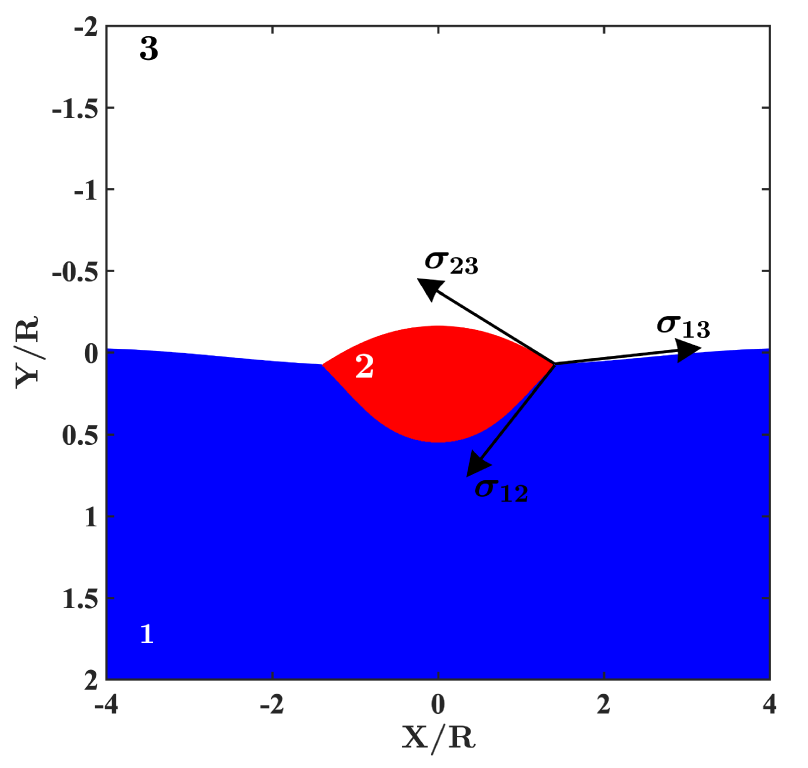
\includegraphics[width=\linewidth]{Schematic}
        \caption{Schematic of the process.}
        \label{Figure:Schematic}
        \end{center}
    \end{minipage}
    \begin{minipage}{0.55\textwidth}
        \begin{center}
        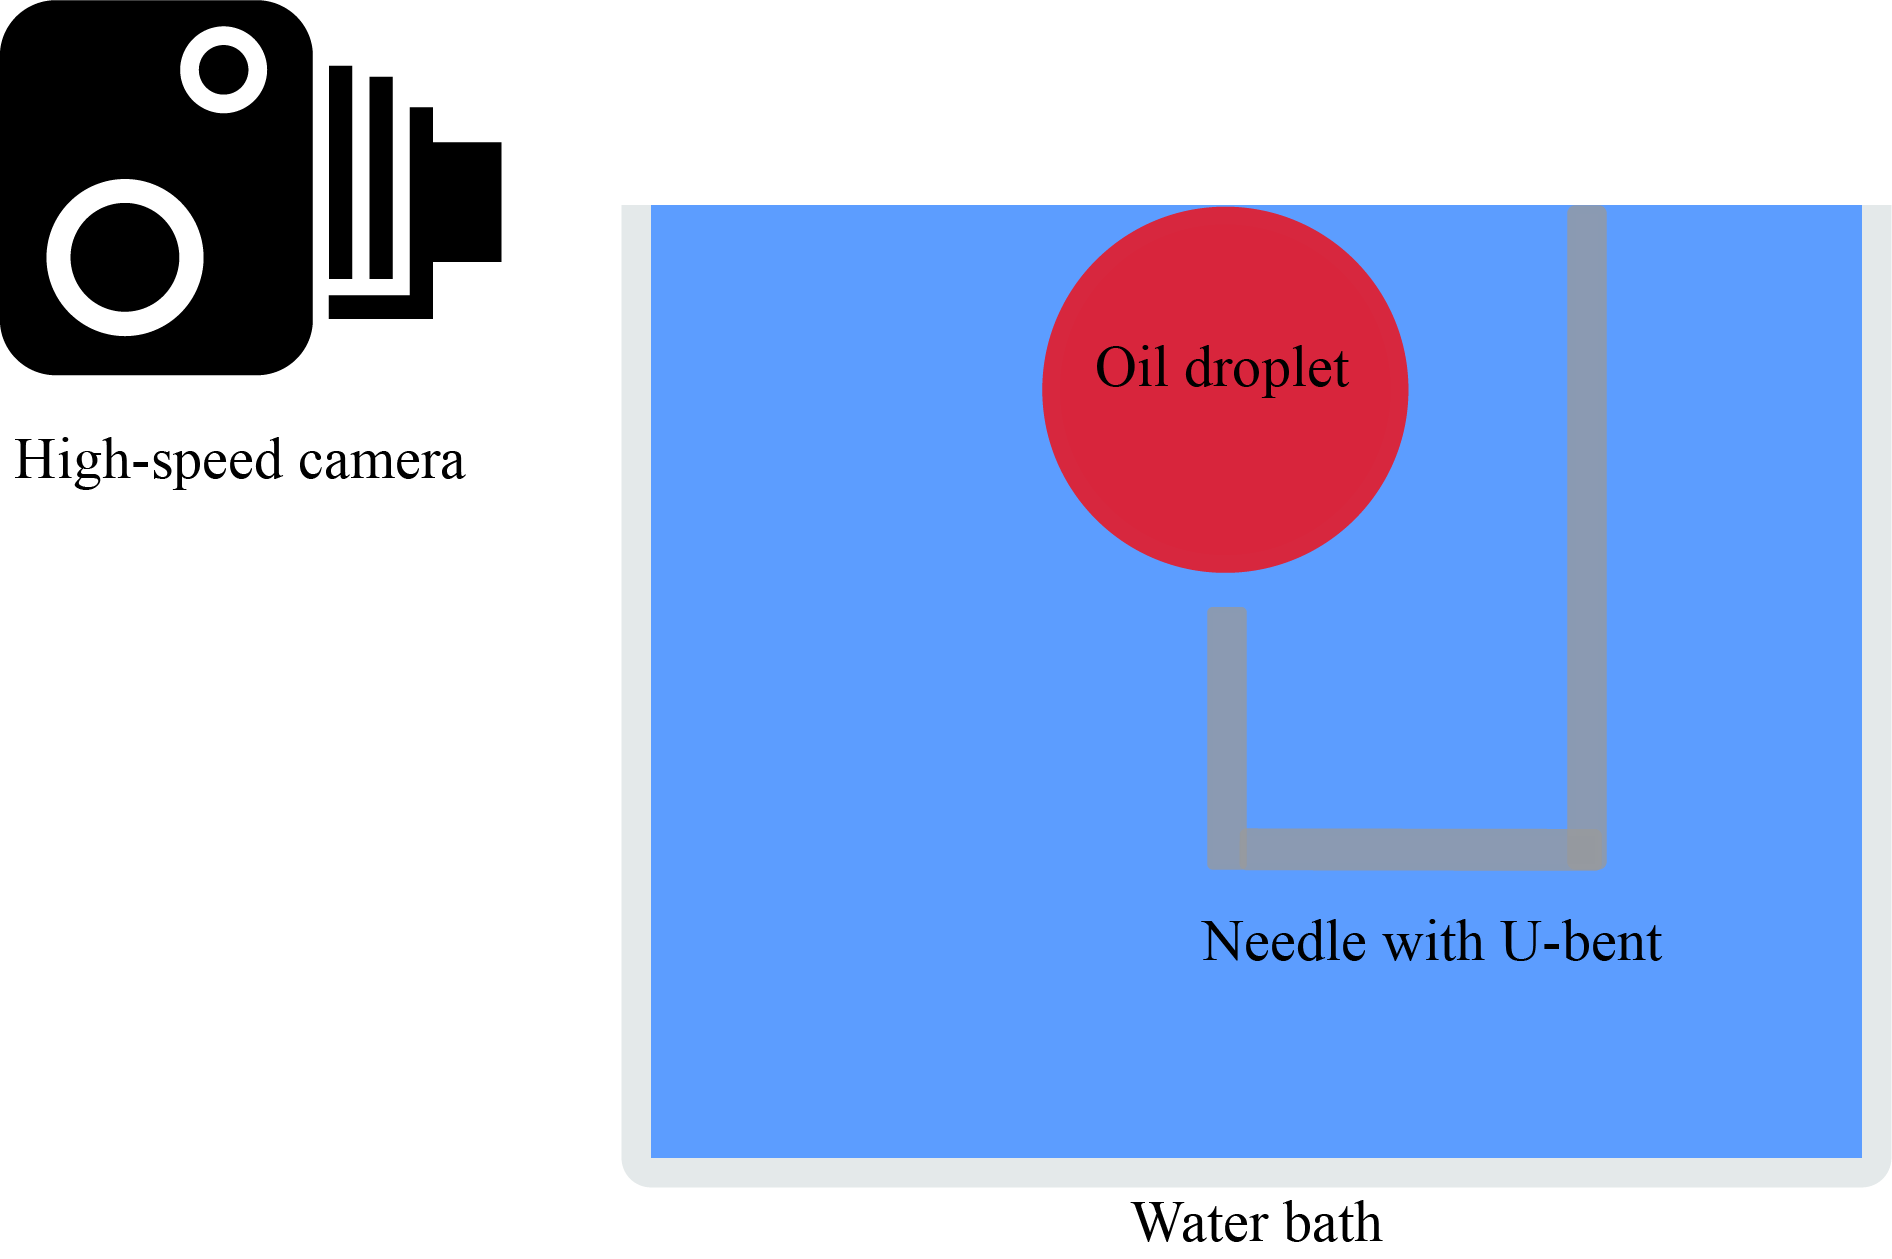
\includegraphics[width=\linewidth]{Experimental_Setup.png}
        \caption{Schematic of the experimental setup.}
        \label{Figure::Experimental}
        \end{center}
    \end{minipage}
\end{figure}
\section*{What will you do \& what will you learn?}
The project will focus on the following:
\begin{enumerate}
\item Design an experiment to visualize spreading of an oil droplet on the water-air interface, as shown schematically in the Figure~\ref{Figure::Experimental}. (\textbf{Skills:} Experimental techniques involving high-speed imaging, fluorescent microscopy, etc.)
\item Determine scaling laws governing the spreading of a droplet on a fluid-fluid interface and compare it with the spreading on a solid surface. (\textbf{Skills:} Fundamentals of two-phase interfacial dynamics.)
\item One to one comparison between experimental results and numerical simulations. (\textbf{Skills:} C/C++ \& Matlab or similar scripting language)
\end{enumerate}
\begin{center}
\begin{tabular}{|l|l|l|l|l|}
\hline \textbf{Supervisor} & \textbf{E-mail} & \textbf{Office} &\textbf{Lab} \\
\hline Dr. P. Kant   & \href{mailto:p.kant@utwente.nl}{p.kant@utwente.nl} & Meander 152 & \\
\hline V. Sanjay & \href{mailto:v.sanjay@utwente.nl}{v.sanjay@utwente.nl} & Meander 212 &\\
\hline Prof. D. Lohse & \href{mailto:d.lohse@utwente.nl}{d.lohse@utwente.nl} & Meander 261  &\\
\hline
\end{tabular}
\end{center}
\printbibliography
\end{document}
